
\section*{Kapitel 1 - Lineare Gleichungssysteme in $\R^n$}

\begin{multicols*}{3}

\tikzstyle{mybox} = [draw=black, fill=white, very thick,
    rectangle, rounded corners, inner sep=10pt, inner ysep=10pt]
\tikzstyle{fancytitle} =[fill=black, text=white, font=\bfseries]

%------------ Lineare Gleichung ---------------
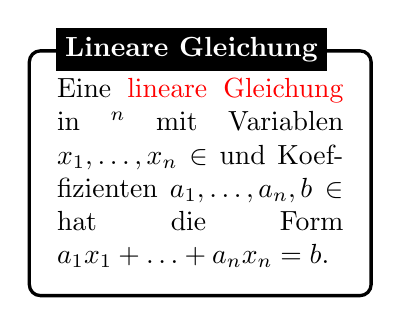
\begin{tikzpicture}
\node [mybox] (box){%
    \begin{minipage}{0.3\textwidth}
    Eine \textcolor{red}{lineare Gleichung} in $\R^n$ mit Variablen $x_1, \dots, x_n \in \R$ und Koeffizienten $a_1, \dots, a_n, b \in \R$ hat die Form $a_1 x_1 + \dots + a_n x_n = b.$
    \end{minipage}
};

%------------ Lineare Gleichung Header ---------------------
\node[fancytitle, right=10pt] at (box.north west) {Lineare Gleichung};
\end{tikzpicture}

%------------ LGS ---------------
\begin{tikzpicture}
\node [mybox] (box){%
    \begin{minipage}{0.3\textwidth}
    Ein \textcolor{red}{lineares Gleichungssystem (LGS)} aus $m$ Gleichungen und $n$ Unbekannten $x_1, \dots, x_n$ hat die Form
	\begin{alignat*}{6}
		 & a_{11} x_1  & {}+{} & \dots           & {}+{} & a_{1n} x_n & {}={} & b_1  \\
		 & a_{21}  x_1 & {}+{} & \dots           & {}+{} & a_{2n} x_n & {}={} & b_2  \\
		 &             &       & \quad \; \vdots                                     \\
		 & a_{m1}  x_1 & {}+{} & \dots           & {}+{} & a_{mn} x_n & {}={} & b_m.
	\end{alignat*}
     Wir nennen zwei LGS \textcolor{red}{äquivalent}, wenn sie die gleichen Lösungen besitzen. Ein LGS lässt sich vollständig durch die Koeffizienten beschreiben und kann daher auch in Form einer \textcolor{red}{(erweiterten) Koeffizientenmatrix} dargestellt werden.
     \begin{align*}
    		\begin{roweqmat}{ccc|c}
    			a_{11} & \dots & a_{1n} & b_1 \\
    			\vdots &   & \vdots & \vdots \\
    			a_{m1} & \cdots & a_{mn} & b_m
    		\end{roweqmat}.
    	\end{align*}
    Ohne die letzte Spalte spricht man von einer Koeffizientenmatrix.
    \end{minipage}
};
%------------ LGS Header ---------------------
\node[text=white, fancytitle, right=10pt] at (box.north west) {Lineares Gleichungssystem};
\end{tikzpicture}

%------------ LGS Beispiel ---------------
\begin{tikzpicture}
\node [mybox] (box){%
    \begin{minipage}{0.3\textwidth}
        \begin{minipage}{0.4\textwidth}
    	\begin{alignat*}{6}
    		 x_1 & {}+{}  & 5x_2 & {}+{} & 3x_3 & {}={} & -2 \\
    		 2x_1 & {}+{} & 2x_2 & {}+{} & 4x_3 & ={} & 8 \\
    		 -3x_1 & {}+{} & 2x_2 & {}+{} & 9x_3 & {}={} & -1
    	\end{alignat*}
    \end{minipage}
    \begin{minipage}{0.4\textwidth}
    	\begin{align*}
    		\qquad \longrightarrow
    	\begin{roweqmat}{rrr|r}
    		1 & 5 & 3 & -2 \\
    		2 & 2 & 4 & 8 \\
    		-3 & 2 & 9 & -1
    	\end{roweqmat}
    \end{align*}
    \end{minipage}
    \end{minipage}
};
%------------ LGS Beispiel Header ---------------------
\node[fill = blue, text=white, font=\bfseries, right=10pt] at (box.north west) {LGS Beispiel};
\end{tikzpicture}

%------------ Elementare Zeilenoperationen ---------------
\begin{tikzpicture}
\node [mybox] (box){%
    \begin{minipage}{0.3\textwidth}
    Um das LGS zu vereinfachen, ohne die Lösungsmenge zu ändern, sind folgende \textcolor{red}{elementare Zeilenoperationen} erlaubt:

	\begin{enumerate}[(i)]
		\item Multipliziere eine Zeile mit einer Konstante \\$c \neq 0$.
		\item Tausche zwei Zeilen.
		\item Addiere eine Zeile $c \neq 0$ mal zu einer anderen.
	\end{enumerate}
    \end{minipage}
};
%------------ Elementare Zeilenoperationen Header ---------------------
\node[fill = purple, text=white, font=\bfseries, right=10pt] at (box.north west) {Elementare Zeilenoperationen};
\end{tikzpicture}

%------------ Zeilenstufenform ---------------
\begin{tikzpicture}
\node [mybox] (box){%
    \begin{minipage}{0.3\textwidth}
    Eine Matrix ist in \textcolor{red}{Zeilenstufenform}, wenn:
	\begin{enumerate}[(i)]
		\item Alle \textcolor{red}{Nullzeilen} (Zeilen, in der höchstens der letzte Eintrag ungleich 0 ist) befinden sich am Ende der Matrix.
		\item Die \textcolor{red}{Pivots} (der erste Eintrag $a_{ji}$ einer Zeile ungleich Null: $j_i = \min\{j\colon a_{ij} \neq 0\})$ der anderen  Zeilen erfüllen die Stufenbedingung
		      $$j_{1} < j_{2} < \dots < j_{r}.$$
        Variablen die zu einer Pivot gehören nennen wir \textcolor{red}{gebunden} und die restlichen Variablen nennen wir \textcolor{red}{frei}
	\end{enumerate}

    Eine Matrix ist in \textcolor{red}{reduzierter Zeilenstufenform}, wenn sie die folgenden Bedingungen erfüllt:
	\begin{enumerate}[(i)]
		\item Sie ist in Zeilenstufenform.
		\item Alle Pivoteinträge $a_{i j_i}$ sind gleich 1.
		\item Alle Spalteneinträge über einem Pivot sind gleich 0.
	\end{enumerate}
    \end{minipage}
};
%------------ Zeilenstufenform Header ---------------------
\node[fill = black, text=white, font=\bfseries, right=10pt] at (box.north west) {(reduzierte) Zeilenstufenform};
\end{tikzpicture}

%------------ LGS Zeilenstufenform Beispiel ---------------
\begin{tikzpicture}
\node [mybox] (box){%
    \begin{minipage}{0.3\textwidth}
    Das untere LGS ist in Zeilenstufenform, aber nicht in reduzierter Zeilenstufenform.\\
    \begin{minipage}{0.4\textwidth}
	\begin{alignat*}{4}
		 & x_1 {}-{} & 2x_2 {}+{} & 6x_3 & {}={} & 2  \\
		 &           & 7x_2 {}+{} & 3x_3 & {}={} & 2  \\
		 &           &            & 3x_3 & {}={} & 2.
	\end{alignat*}
\end{minipage}
\begin{minipage}{0.4\textwidth}
	\begin{align*}
		\qquad \longrightarrow
	\begin{roweqmat}{rrr|r}
		1 & -2 & 6 & 2 \\
		0 & 7 & 3 & 2 \\
		0 & 0 & 3 & 2
	\end{roweqmat}
\end{align*}
\end{minipage}
    \end{minipage}
};
%------------ LGS Zeilenstufenform Beispiel Header ---------------------
\node[fill = blue, text=white, font=\bfseries, right=10pt] at (box.north west) {LGS in Zeilenstufenform};
\end{tikzpicture}

%------------ Anzahl Lösungen ---------------
\begin{tikzpicture}
\node [mybox] (box){%
    \begin{minipage}{0.3\textwidth}
    \begin{enumerate}[(i)]
		\item 	Ein LGS hat genau dann keine Lösung, wenn sich durch elementare Zeilenoperationen eine \emph{Nullzeile}
		      $$ \begin{roweqmat}{rrrr|c} 0 & 0 & \cdots & 0 & c \end{roweqmat} $$
		      mit $c \neq 0$ erzeugen lässt.
		\item Ein lösbares LGS hat genau eine Lösung, wenn es keine freien Variablen gibt. Andernfalls gibt es unendlich viele Lösungen.
	\end{enumerate}
    \end{minipage}
};
%------------ Anzahl Lösungen Header ---------------------
\node[fill = purple, text=white, font=\bfseries, right=10pt] at (box.north west) {Anzahl Lösungen};
\end{tikzpicture}

%------------ Elementare Zeilenoperationen Beispiele---------------
\begin{tikzpicture}
\node [mybox] (box){%
    \begin{minipage}{0.3\textwidth}
    \begin{eqnarray*}
		& & \begin{roweqmat}{rrr|c}
			3 & 6 & -6 & 3 \\
			1 & 2 & 0 & 3 \\
			-2 & -1 & 9 & -2
		\end{roweqmat} \\
		&  \stackrel{\frac13 \cdot (1)}{\sim} &
		\begin{roweqmat}{rrr|c}
			1 & 2 & -2 & 1 \\
			1 & 2 & 0 & 3 \\
			-2 & -1 & 9 & -2
		\end{roweqmat}
		\\
		& \stackrel{(2) - (1)}{\sim} &
		\begin{roweqmat}{rrr|c}
			1 & 2 & -2 & 1 \\
			0 & 0 & 2 & 2 \\
			-2 & -1 & 9 & -2
		\end{roweqmat}
		\\
		& \stackrel{(2)\leftrightarrow (3)}{\sim} &
		\begin{roweqmat}{rrr|c}
			1 & 2 & -2 & 1 \\
			-2 & -1 & 9 & -2  \\
			0 & 0 & 2 & 2
		\end{roweqmat}
		\\
		& \stackrel{(2) + 2 \cdot (1)}{\sim}	&
		\begin{roweqmat}{rrr|c}
			1 & 2 & -2 & 1 \\
			0 & 3 & 5 & 0 \\
			0 & 0 & 2 & 2
		\end{roweqmat}.
	\end{eqnarray*}
 Jetzt ist die erweiterte Koeffizientenmatrix in Zeilenstufenform.
    \begin{eqnarray*}
		&  \stackrel{\frac13 \cdot (2)}{\sim} &
		\begin{roweqmat}{rrr|c}
			1 & 2 & -2 & 1 \\
			0 & 1 & \frac53 & 0 \\
			0 & 0 & 2 & 2
		\end{roweqmat}
		\\
		& \stackrel{(1) - 2\cdot(2)}{\sim} &
		\begin{roweqmat}{rrr|c}
			1 & 0 & -\frac{16}{3}  & 1 \\
			0 & 1 & \frac53 & 0 \\
			0 & 0 & 2 & 2
		\end{roweqmat}
		\\
		& \stackrel{\frac12 \cdot (3)}{\sim} &
		\begin{roweqmat}{rrr|c}
			1 & 0 & -\frac{16}{3}  & 1 \\
			0 & 1 & \frac53 & 0 \\
			0 & 0 & 1 & 1
		\end{roweqmat}
		\\
		& \stackrel{(1) + \frac{16}{3} \cdot (3)}{\sim}	&
		\begin{roweqmat}{rrr|c}
			1 & 0 & 0 & \frac{19}{3} \\
			0 & 1 & \frac53 & 0 \\
			0 & 0 & 1 & 1
		\end{roweqmat}
        \\
		& \stackrel{(2) - \frac{5}{3} \cdot (3)}{\sim}	&
		\begin{roweqmat}{rrr|c}
			1 & 0 & 0 & \frac{19}{3} \\
			0 & 1 & 0 & - \frac53 \\
			0 & 0 & 1 & 1
		\end{roweqmat}
	\end{eqnarray*}
    Jetzt ist die erweiterte Koeffizientenmatrix in reduzierter Zeilenstufenform.
    \end{minipage}
};
%------------ Elementare Zeilenoperationen Beispiele Header---------------------
\node[fill = blue, text=white, font=\bfseries, right=10pt] at (box.north west) {Elementare Zeilenoperationen Beispiel};
\end{tikzpicture}

%------------ Gauss-Jordan-Verfahren ---------------
\begin{tikzpicture}
\node [mybox] (box){%
    \begin{minipage}{0.3\textwidth}
    Um die Lösungen von einem LGS zu bestimmen, kann man das Gauss-Jordan-Verfahren benutzen:
    \begin{enumerate}[(i)]
	\item Schreibe das LGS in eine Koeffizientenmatrix.
	\item Bringe Matrix durch elementare Zeilenoperationen in Zeilenstufenform.
	\item Stelle fest, ob das System lösbar ist.
	\item Falls ja, reduziere die Matrix um Lösungen zu bestimmen.
\end{enumerate}
    \end{minipage}
};
%------------ Gauss-Jordan-Verfahren Header ---------------------
\node[fill = mycolor, text=white, font=\bfseries, right=10pt] at (box.north west) {Gauss-Jordan-Verfahren};
\end{tikzpicture}


%------------ Vektor in \R^n ---------------
\begin{tikzpicture}
\node [mybox] (box){%
    \begin{minipage}{0.3\textwidth}
    Ein \tc{$n$-dimensionaler Vektor} ist ein geordnetes $n$-Tupel $\bx = (x_1, \dots, x_n)$ von reellen Zahlen $x_1, \dots, x_n \in \R$, genannt Komponenten.
    \begin{itemize}
	\item Wir schreiben $\bx \in \R^n$ in Spaltenform:
	      $$ \bx = \begin{pmatrix}
			      x_1 \\ \vdots \\ x_n
		      \end{pmatrix}.$$
	\item $\bx = \by  \equivto \  x_i = y_i \mbox{ für alle } i = 1, \dots, n.$
	     
	\item 	Wir definieren den \tc{Nullvektor} als
	      $$\bm 0 = (\underbrace{0, 0, 0, \dots}_{n \mbox{ \scriptsize{mal}}}),$$
	      und den $j$-ten \tc{Einheitsvektor} als
	      $$\be_j = (0, \dots, 0, \underbrace{1}_{j\mbox{\scriptsize{-te Stelle}}}, 0, \dots, 0).$$
    \item Vektoraddition:
		      $$\bx + \by =\begin{pmatrix}
				      x_1 \\ \vdots \\ x_n
			      \end{pmatrix} + \begin{pmatrix}
				      y_1 \\ \vdots \\  y_n
			      \end{pmatrix} := \begin{pmatrix}
				      x_1 + y_1 \\ \vdots \\ x_n + y_n
			      \end{pmatrix}.$$
	\item Multiplikation mit einem \textbf{Skalar} $\lambda \in \R$:
		      $$ \lambda \cdot \bx := \begin{pmatrix}
				      \lambda \cdot x_1 \\ \vdots \\ \lambda \cdot x_n
			      \end{pmatrix}.$$
    \end{itemize}
    \end{minipage}
};
%------------ Vektor in \R^n Header ---------------------
\node[fill = black, text=white, font=\bfseries, right=10pt] at (box.north west) {Vektor in $\R^n$};
\end{tikzpicture}


%------------ Standardraum ---------------
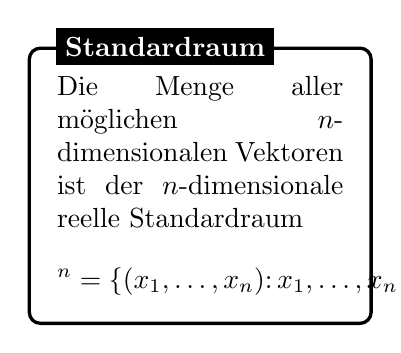
\begin{tikzpicture}
\node [mybox] (box){%
    \begin{minipage}{0.3\textwidth}
    Die Menge aller möglichen $n$-dimensionalen Vektoren ist der \tc{$n$-dimensionale reelle Standardraum}
	$$\R^n = \{(x_1, \dots, x_n)\colon x_1, \dots, x_n \in \R \}.$$
    \end{minipage}
};
%------------ Standardraum Header ---------------------
\node[fill = black, text=white, font=\bfseries, right=10pt] at (box.north west) {Standardraum};
\end{tikzpicture}



%------------ Vektorrechenregeln ---------------
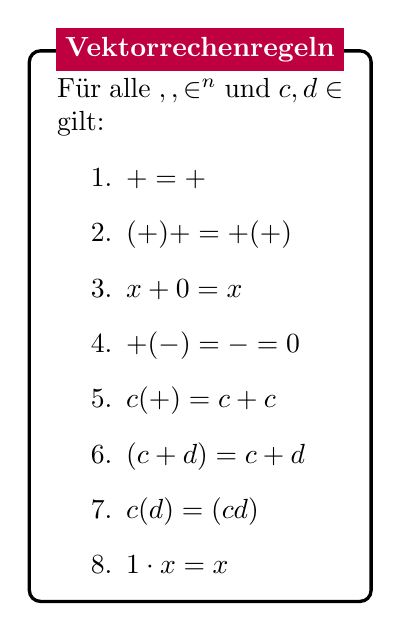
\begin{tikzpicture}
\node [mybox] (box){%
    \begin{minipage}{0.3\textwidth}
    Für alle $\bx, \by, \bz \in \R^n$ und $c, d \in \R$ gilt:
	\begin{enumerate}
		\item $\bx + \by = \by + \bx$
		\item $(\bx + \by) + \bz = \bx + (\by + \bz)$
		\item $\bm x + \bm 0 = \bm x$
		\item $\bx + (-\bx) = \bx - \bx = \bm 0$
		\item $c(\bx + \by) = c\bx  + c\by$
		\item $(c + d)\bx = c\bx + d\bx$
		\item $c(d\bx) = (cd) \bx$
		\item $1 \cdot \bm x = \bm x$
	\end{enumerate}
    \end{minipage}
};
%------------ Vektorrechenregeln Header ---------------------
\node[fill = purple, text=white, font=\bfseries, right=10pt] at (box.north west) {Vektorrechenregeln};
\end{tikzpicture}

%------------ Linearkombinationen ---------------
\begin{tikzpicture}
\node [mybox] (box){%
    \begin{minipage}{0.3\textwidth}
    Wir nennen einen Vektor $\bb \in \R^n$ eine \tc{Linearkombination} von Vektoren $\ba_1, \dots, \ba_k$, wenn er sich als
	$$\bb = c_1 \ba_1 + \cdots + c_k \ba_k$$
	mit $c_1, \dots, c_k \in \R$ schreiben lässt.
	Die Zahlen $c_1, \dots, c_k$ nennen wir Gewichte oder Koeffizienten.
    \end{minipage}
};
%------------ Linearkombinationen Header ---------------------
\node[fill = black, text=white, font=\bfseries, right=10pt] at (box.north west) {Linearkombinationen};
\end{tikzpicture}

%------------ Linearkombinationen Beispiel ---------------
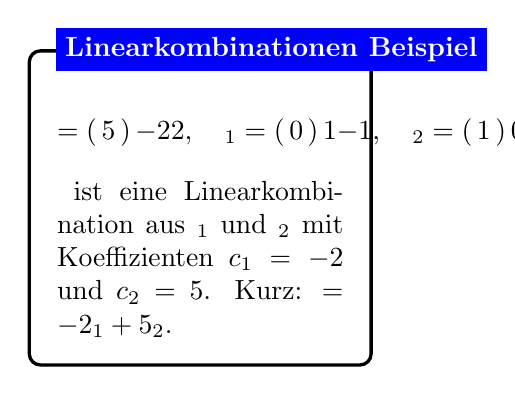
\begin{tikzpicture}
\node [mybox] (box){%
    \begin{minipage}{0.3\textwidth}
	$$\bb = \begin{pmatrix}
			5 \\ -2 \\ 2
		\end{pmatrix}, \quad \ba_1 = \begin{pmatrix}
			0 \\ 1 \\ -1
		\end{pmatrix}, \quad \ba_2 = \begin{pmatrix}
			1 \\ 0 \\ 0
		\end{pmatrix}.$$
	$\bb$ ist eine Linearkombination aus $\ba_1$ und $\ba_2$ mit Koeffizienten $c_1 = -2$ und $c_2 = 5$. Kurz: $\bb = -2 \ba_1 + 5 \ba_2$.
    \end{minipage}
};
%------------ Linearkombinationen Beispiel Header ---------------------
\node[fill = blue, text=white, font=\bfseries, right=10pt] at (box.north west) {Linearkombinationen Beispiel};
\end{tikzpicture}

%------------ Spann ---------------
\begin{tikzpicture}
\node [mybox] (box){%
    \begin{minipage}{0.3\textwidth}
    Die Menge aller Linearkombinationen von gegeben Vektoren $\ba_1, \dots, \ba_k \in \R^n$ bezeichnen wir als \tc{Spann} oder die von den Vektoren \tc{aufgespannte Menge}:
	$$\spann\{\ba_1, \dots, \ba_k\} = \{ c_1 \ba_1 + \cdots + c_k \ba_k\colon c_1, \dots, c_k \in \R\}.$$
    \end{minipage}
};
%------------ Spann Header ---------------------
\node[fill = black, text=white, font=\bfseries, right=10pt] at (box.north west) {Spann};
\end{tikzpicture}

%------------ Lemma zum Spann ---------------
\begin{tikzpicture}
\node [mybox] (box){%
    \begin{minipage}{0.3\textwidth}
    \begin{enumerate}[(i)]
		\item $\bm 0 \in \spann\{\ba_1, \dots, \ba_k\}$,
		\item $\bm \ba_i \in \spann\{\ba_1, \dots, \ba_k\}$ für alle $i = 1, \dots, k$,
		\item LGS $(\ba_1 \quad \cdots \quad \ba_k \mid \bb)$ hat eine Lösung \\$\equivto \bb \in \spann\{\ba_1, \dots, \ba_k\}$ 
	\end{enumerate}
    \end{minipage}
};
%------------ Lemma zum Spann Header ---------------------
\node[fill = purple, text=white, font=\bfseries, right=10pt] at (box.north west) {Lemma zum Spann};
\end{tikzpicture}

%------------ Spann Visualisierung ---------------
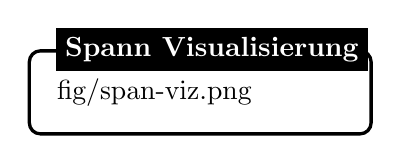
\begin{tikzpicture}
\node [mybox] (box){%
    \begin{minipage}{0.3\textwidth}
    \fig{fig/span-viz.png}
    \end{minipage}
};
%------------ Spann Visualisierung Header ---------------------
\node[fill = black, text=white, font=\bfseries, right=10pt] at (box.north west) {Spann Visualisierung};
\end{tikzpicture}

%------------ Matrix ---------------
\begin{tikzpicture}
\node [mybox] (box){%
    \begin{minipage}{0.3\textwidth}
    Eine rechteckiges Schema mit $m$ Zeilen und $n$ Spalten gefüllt mit reellen Zahlen $a_{ij} \in \R$,
	$$A = \begin{pmatrix}
			a_{11} & \cdots & a_{1n} \\
			\vdots &        & \vdots \\
			a_{m1} & \cdots & a_{mn} \\
		\end{pmatrix},$$
	bezeichnen wir als \tc{$(m \times n)$-Matrix} und schreiben $A \in \R^{m \times n}$.
    \end{minipage}
};
%------------ Matrix Header ---------------------
\node[fill = black, text=white, font=\bfseries, right=10pt] at (box.north west) {Matrix};
\end{tikzpicture}

%------------ Matrix-Vektor-Produkt ---------------
\begin{tikzpicture}
\node [mybox] (box){%
    \begin{minipage}{0.3\textwidth}
    Das \tc{Matrix-Vektor-Produkt} von $A \in \R^{m \times n}$ mit Spalten $\ba_1, \dots, \ba_n$ und $\bm x \in \R^n$ ist definiert als
	$$A \bx = x_1 \ba_1 + \cdots + x_n \ba_n.$$
    \end{minipage}
};
%------------ Matrix-Vektor-Produkt Header ---------------------
\node[fill = black, text=white, font=\bfseries, right=10pt] at (box.north west) {Matrix-Vektor-Produkt};
\end{tikzpicture}


%------------ Matrix-Vektor-Produkt Beispiel ---------------
\begin{tikzpicture}
\node [mybox] (box){%
    \begin{minipage}{0.3\textwidth}
    $\begin{pmatrix}
			1 & 2  \\
			3 & -2 \\
			0 & 1
		\end{pmatrix} \begin{pmatrix}
			1 \\ -4
		\end{pmatrix} = 1 \cdot \begin{pmatrix}
			1 \\ 3 \\ 0
		\end{pmatrix} - 4 \cdot\begin{pmatrix}
			2 \\ -2 \\ 1
		\end{pmatrix}
        = \begin{pmatrix}
			-7 \\ 11 \\ -4
		\end{pmatrix} $
    \end{minipage}
};
%------------ Matrix-Vektor-Produkt Beispiel Header ---------------------
\node[fill = blue, text=white, font=\bfseries, right=10pt] at (box.north west) {Matrix-Vektor-Produkt Beispiel};
\end{tikzpicture}


%------------ Rechenregeln Matrix-Vektor-Produkt ---------------
\begin{tikzpicture}
\node [mybox] (box){%
    \begin{minipage}{0.3\textwidth}
    Sei $A \in \R^{m \times n}$, $\bx, \by \in \R^n$ und $c \in \R$. Dann gilt:
	\begin{enumerate}[(i)]
		\item $A(\bx + \by) = A\bx + A\by$,
		\item $A(c\bx) = c(A\bx)$.
	\end{enumerate}
    \end{minipage}
};
%------------ Rechenregeln Matrix-Vektor-Produkt Header ---------------------
\node[fill = purple, text=white, font=\bfseries, right=10pt] at (box.north west) {Rechenregeln Matrix-Vektor-Produkt};
\end{tikzpicture}

%------------ (in)homogenes LGS ---------------
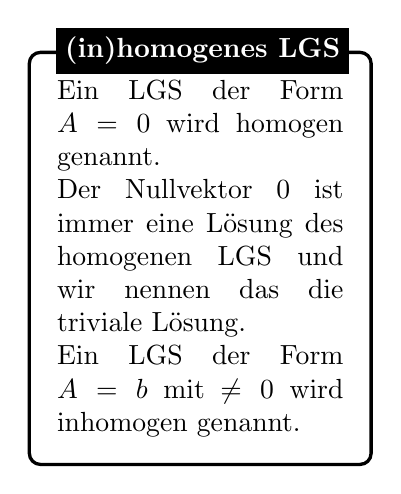
\begin{tikzpicture}
\node [mybox] (box){%
    \begin{minipage}{0.3\textwidth}
		Ein LGS der Form $A\bx = \bm 0$ wird \tc{homogen} genannt.\\
		Der Nullvektor $\bm 0$ ist immer eine Lösung des homogenen LGS und wir nennen das die \tc{triviale Lösung}.\\
		Ein LGS der Form $A\bx = \bm b$ mit $\bb \neq \bm 0$ wird \tc{inhomogen} genannt.
    \end{minipage}
};
%------------ (in)homogenes LGS Header ---------------------
\node[fill = black, text=white, font=\bfseries, right=10pt] at (box.north west) {(in)homogenes LGS};
\end{tikzpicture}


%------------ Lösungsmenge homogener LGS ---------------
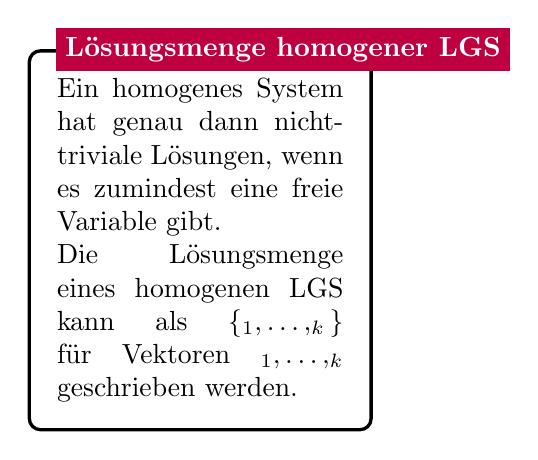
\begin{tikzpicture}
\node [mybox] (box){%
    \begin{minipage}{0.3\textwidth}
		Ein homogenes System hat genau dann nicht-triviale Lösungen, wenn es zumindest eine freie Variable gibt.\\
		Die Lösungsmenge eines homogenen LGS kann als $\spann\{\bv_1, \dots, \bv_k\}$ für Vektoren $\bv_1, \dots, \bv_k$ geschrieben werden.
    \end{minipage}
};
%------------ Lösungsmenge homogener LGS Header ---------------------
\node[fill = purple, text=white, font=\bfseries, right=10pt] at (box.north west) {Lösungsmenge homogener LGS};
\end{tikzpicture}

%------------ Lösungsmenge inhomogener LGS ---------------
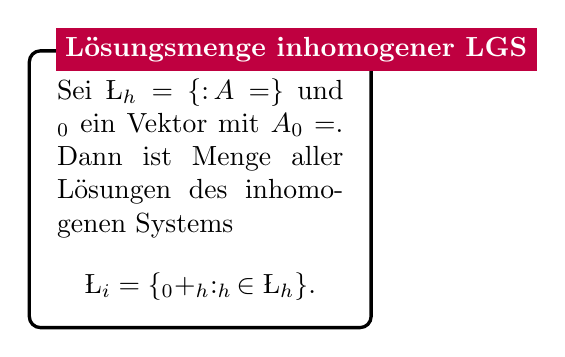
\begin{tikzpicture}
\node [mybox] (box){%
    \begin{minipage}{0.3\textwidth}
    Sei $\L_h = \{\bx \colon A\bx = \bnull\}$ und $\bx_0$ ein Vektor mit  $A\bx_0 = \bb$. Dann ist Menge aller Lösungen des inhomogenen Systems
  	$$\L_i = \{\bx_0 + \bx_h\colon \bx_h \in \L_h\}.$$
    \end{minipage}
};
%------------ Lösungsmenge inhomogener LGS Header ---------------------
\node[fill = purple, text=white, font=\bfseries, right=10pt] at (box.north west) {Lösungsmenge inhomogener LGS};
\end{tikzpicture}

%------------ Lösungsmenge inhomogener LGS Beispiel ---------------
\begin{tikzpicture}
\node [mybox] (box){%
    \begin{minipage}{0.3\textwidth}
    Wir betrachten das folgende LGS in reduzierter Zeilenstufen
	\begin{align*}
    \begin{roweqmat}{rrrr|c}
      1 & 0 & 3 & 0 & 1 \\
      0 & 1 & -2 & 5 & -4 \\
      0 & 0 & 0 & 0 & 0
    \end{roweqmat}
  	\end{align*}
	was wir wiefolgt ausdrücken können:
	$$\begin{array}{rrrrrrr}
      x_1 & = & 1 & + & - 3x_3 & + & 0x_4 \\
      x_2 & = & -4 & + & 2x_3   & + & -5x_4 \\
      x_3 & = & 0 & + & 1x_3   & + & 0x_4 \\
      x_4 & = & 0 & + & 0x_3   & + & 1x_4
    \end{array}.$$
	Damit lässt jeder Lösungsvektor schreiben als
	\begin{align*}
		\begin{pmatrix}
		  x_1 \\ x_2 \\ x_3 \\ x_4
		\end{pmatrix} = \begin{pmatrix}
			1 \\ -4 \\ 0 \\ 0
		  \end{pmatrix} + c_3 \begin{pmatrix}
		  -3 \\ 2 \\ 1 \\ 0
		\end{pmatrix} + c_4 \begin{pmatrix}
		  0 \\ -5 \\ 0 \\ 1
		\end{pmatrix}, \quad c_3, c_4 \in \R,
	  \end{align*}
	  Wenn wir die rechte Seite zu $\bm 0$ ändern, dann lässt sich die Lösungsmenge schreiben als
	  \begin{align*}
		\L_h = \spann\biggl\{\begin{pmatrix}
		  -3 \\ 2 \\ 1 \\ 0
		\end{pmatrix}, 
		\begin{pmatrix}
		  0 \\ -5 \\ 0 \\ 1
		\end{pmatrix} \biggr\}.
	  \end{align*}
    \end{minipage}
};
%------------ Lösungsmenge inhomogener LGS Beispiel Header ---------------------
\node[fill = blue, text=white, font=\bfseries, right=10pt] at (box.north west) {Lösungsmenge (in)homogener LGS Beispiel};
\end{tikzpicture}

%------------ Lineare (Un)Abhängigkeit ---------------
\begin{tikzpicture}
\node [mybox] (box){%
    \begin{minipage}{0.3\textwidth}
    Eine Menge von Vektoren $\bv_1, \dots, \bv_k \in \R^n$ sind \tc{linear unabhängig}, wenn die Vektorgleichung
  	$$x_1 \bv_1 + \cdots + x_k \bv_k = \bnull$$
  	nur die triviale Lösung $\bx = \bnull$ besitzt. Andernfalls nennen wir die Vektoren \tc{linear abhängig}.
    \end{minipage}
};
%------------ Lineare (Un)Abhängigkeit Header ---------------------
\node[fill = black, text=white, font=\bfseries, right=10pt] at (box.north west) {Lineare (Un)Abhängigkeit};
\end{tikzpicture}

%------------ Lineare (Un)Abhängigkeit ---------------
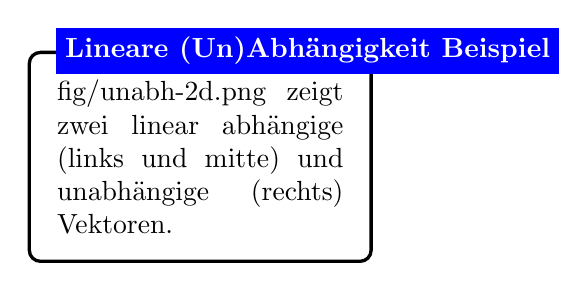
\begin{tikzpicture}
\node [mybox] (box){%
    \begin{minipage}{0.3\textwidth}
    \fig{fig/unabh-2d.png}
	zeigt zwei linear abhängige (links und mitte) und unabhängige (rechts) Vektoren.
    \end{minipage}
};
%------------ Lineare (Un)Abhängigkeit Header ---------------------
\node[fill = blue, text=white, font=\bfseries, right=10pt] at (box.north west) {Lineare (Un)Abhängigkeit Beispiel};
\end{tikzpicture}


%------------ Lineare (Un)Abhängigkeit Theorem ---------------
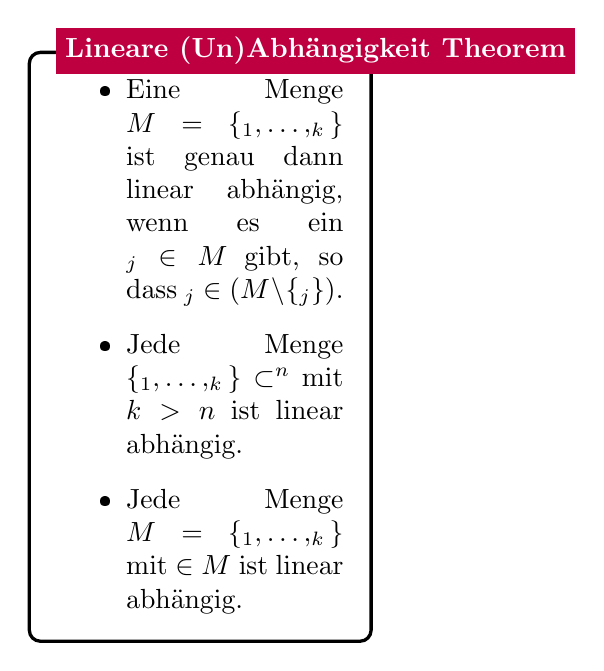
\begin{tikzpicture}
\node [mybox] (box){%
    \begin{minipage}{0.3\textwidth}
	\begin{itemize}
    \item Eine Menge $M = \{\bv_1, \dots, \bv_k\}$ ist genau dann linear abhängig, wenn es ein $\bv_j \in M$ gibt, so dass 	$\bv_j \in \spann(M \setminus \{\bv_j\})$.
	\item Jede Menge $\{\bv_1, \dots, \bv_k\} \subset \R^n$ mit $k > n$ ist linear abhängig.
	\item Jede Menge $M = \{\bv_1, \dots, \bv_k\}$ mit $\bnull \in M$ ist linear abhängig.
	\end{itemize}
    \end{minipage}
};
%------------ Lineare (Un)Abhängigkeit Theorem Header -----------------
\node[fill = purple, text=white, font=\bfseries, right=10pt] at (box.north west) {Lineare (Un)Abhängigkeit Theorem};
\end{tikzpicture}



%------------ Megatheorem ---------------
\begin{tikzpicture}
\node [mybox] (box){%
    \begin{minipage}{0.3\textwidth}
    Sei $A \in \R^{m \times n}$. Die folgenden Aussagen sind äquivalent:
	\begin{enumerate}[(i)]
		\item $A \bx = \bb$ hat eine Lösung für jedes $\bb \in \R^m$.
		\item Jedes $\bb \in \R^m$ ist eine Linearkombination der Spalten von $A$.
		\item $\spann\{\ba_1, \dots, \ba_n\} = \R^m$.
		\item $A$ hat ein Pivot in jeder Zeile.
	\end{enumerate}
    \end{minipage}
};
%------------ Megatheorem Header ---------------------
\node[fill = purple, text=white, font=\bfseries, right=10pt] at (box.north west) {Megatheorem};
\end{tikzpicture}


%------------ Überschrift ---------------

\begin{tikzpicture}
\node [mybox] (box){%
    \begin{minipage}{0.3\textwidth}
    
    \end{minipage}
};
%------------ Überschrift Header ---------------------
\node[fill = black, text=white, font=\bfseries, right=10pt] at (box.north west) {Überschrift};
\end{tikzpicture}

\end{multicols*}



